In this section, we compare $\latentranker$ to several bandit algorithms in three experiments. The first two experiments are on synthetic problems where all modeling assumptions hold. The third experiment is on a real-world dataset where we evaluate $\latentranker$ when our modeling assumptions fail. All results are averaged over $10$ independent random runs. We test in both rank $1$ and rank $2$ settings to clearly illustrate the failures of the current rank $1$ algorithms and show the efficiency of our proposed method. 

%We use the term rows/users and columns/items interchangeably. 

%\todob{You already said this before multiple times. What are users and items really buying us? We should call rows ``rows'' and columns ``columns''. In our motivating example, the columns are marketing channels. Item does not sound like the right analogue.}
%In all our experiments user come uniform randomly over all time $[n]$. 

%\subsection{Evaluated Algorithms for Rank-$1$}
\subsection{Experiments on Rank-$1$ Setting}

\textbf{Evaluated Algorithms for Rank-$1$:} We compare against several state-of-the-art rank $1$ algorithms. Note that all the rank $1$ algorithms suggest a single row and column at every round. The $\ucb$ algorithm from \citet{auer2002finite} builds a confidence set at every round $t$ over all the entries of $M_t$ as $c_{i, j}(t) = \sqrt{\frac{2\log t}{N_{i, j}(t)}}$ where $N_{i, j}(t)$ denotes the number of times the $(i,j)$-th entry has been observed. It the suggests the best row-column pair based on the term $\hat{M}_{t}(i,j) + c_{i, j}(t)$ where $\hat{M}_{t}(i,j)$ is the empirical mean of all observed rewards of entry $(i,j)$. The $\ucbe$ \citep{auer2010ucb} is similar to $\ucb$ but it eliminates sub-optimal rows and columns  based on a similar confidence set  $c_{i, j}(t)$ till it finally converges on the best pair of row and column. The algorithm $\linucb$ was first proposed in \citet{li2010contextual} for the contextual bandit setting. Note that rank-$1$ bandit generalizes to the stochastic linear bandit setting and can be solved by $\linucb$. Similarly, GLM-UCB from \citet{filippi2010parametric} can also be used to solve the rank-$1$ bandit problem. Finally, we compare against the algorithm $\rankelim$ from \citet{katariya2016stochastic} which is an improved version of $\ucbe$ and employs row and column elimination and aggressive exploration to converge on the best row and column pair. For $\latentranker$ we use the Algorithm \ref{alg:LRB} from Section \ref{sec:rank1}. We use eq \eqref{eq:regret} definition to calculate regret in rank-$1$ setting.

%which computes the maximum-likelihood estimates of the parameter vector $\theta \in \{0,1\}^{K+L}$ (using Expectation-Maximization algorithm)
%\todob{I do not think that this is true.}
%We use \expthree as the \rowalg and \colalg with the exploration parameter $\gamma_{\text{\rowalg}} = \sqrt{\frac{K\log K}{T}}$ and $\gamma_{\text{\colalg}} = \sqrt{\frac{L\log L}{T}}$ respectively.
% \todob{Weird hyphen. Use mhyphen instead.}
%, that \todoan{I don't think you need a ',' between 'Note' and 'that'. This repeats in at least a couple of places.}
%\todob{Restructure this section as follows. Baselines for rank $1$. Rank $1$ results. Algorithms for rank $2$. Rank $2$ results. It is too early to talk about rank $2$ algorithms before you should rank $1$ results.}
%\subsection{Synthetic Experiment $1$ for Rank-$1$}
\textbf{Synthetic Experiment $1$ for Rank-$1$:} This experiment is conducted to test the performance of $\latentranker$ over a small number of rows and columns and to show how $\latentranker$ scales with increasing number of rows and columns. Note that in this experiment all our modeling assumptions hold. This simulated testbed consist of two scenarios: (1) $8$ rows and $8$ columns and (2) $16$ rows and $16$ columns. In this setting, $U = \{0.7, 0.9\}^{K\times 1}$ and similarly $V = \{0.7, 0.9\}^{L\times 1}$ with only the entry $U(K/2,1) = V(L/2,1) = 0.9$. Hence, the matrix $M = UV^{\intercal}$ is rank $1$ and the hott-topics structure is maintained. At every round $t$, we generate the matrix $M_t = UD_tV^{\intercal}$ where $D_t$ is a randomly generated value from $[0,1]$. Note for all round $t\in [n]$, $M_t$ is rank-$1$ matrix with its maximum value always at $M_t(K/2,L/2)$, and other entries changing arbitrarily but always less than $M_t(K/2,L/2)$. The learner observes the entry $M_t(i,j)$ when it selects the $i$-th row and $j$-th column. A similar environment has been discussed as $B_{\text{spike}}$ in \citet{katariya2016stochastic}. From Figure \ref{fig:1} and \ref{fig:2} we can clearly see that $\latentranker$ outperforms all the other algorithms. The regret curve of $\latentranker$ flattens, indicating that it has learned the best row-column pair. As we scale the number of rows and columns we see that $\latentranker$ performs even better than other algorithms. 

\subsection{Experiments on Rank-$2$ Setting}

\textbf{Evaluated Algorithms for Rank-$2$:} We design the rank-$2$ algorithms by modifying the rank-$1$ algorithms. Again note that all the rank-$2$ algorithms suggest two pairs of rows and columns at every round $t$. For all of the algorithms $\ucb$, $\ucbe$, $\linucb$, $\glmucb$, and $\rankelim$ we modify these algorithms so that they suggest $2$ pairs of rows and columns based on their respective confidence interval set $c_{i, j}(t)$. The row and column pair with the highest and the second highest $\hat{M}_{t}(i,j) + c_{i, j}(t)$ are suggested for each round $t$ and consequently after observing all the entries of $M_t(i,j)$ all of the algorithms update their estimates of $\hat{M}_{t}(i,j)$ for each $i,j \in [d]$. For $\latentranker$ we use the Algorithm \ref{alg:LRB1} from Section \ref{sec:algorithm}. Note that there are two $\rowalg$ and $\colalg$, each running a $\expthree$ algorithm with the exploration parameters as discussed before. For $\latentranker$-rank$2$ we use the Algorithm \ref{alg:LRB1} from Section \ref{sec:algorithm}. We also modify the rank-$1$ $\latentranker$ (Algorithm \ref{alg:LRB}) so that the algorithm works in rank-$2$ setting. After $\latentranker$-rank$1$ has sampled one pair of rows and columns from $[K]$ and $[L]$, it then samples again another choice that does not clash with the first pair and then updates all the pairs with the feedback observed. We use eq \eqref{eq:regret1} definition to calculate regret in rank-$2$ setting.



%$u_t(i)$ is an independent Bernoulli variable with mean $U(i,1)$ and $v_t(j)$ is an independent Bernoulli variable with mean $V(j,1)$.
%\todoan{Why do our assumptions hold in this experiment? You sample a Bernoulli outcome, so the optimal row/column can change across time steps.}
%$u_t = \mathcal{D} + \Delta_u$ and $v_t =  \mathcal{D}_t  + \Delta_v$, where $\mathcal{D}_t \in \{0,1\}$ is independent Bernoulli noise and $\Delta_u = \Delta_v = 0.2$
%Independent user model algorithms $\RBAUCB$ and $\RBAEXP$  perform poorly as the number of items per user is too large and the independent algorithms are not sharing information between them. $\NMFBan$ performs better than the independent user model algorithms but is outperformed by $\LRAEXP$, $\LRATS$ and $\LRAUCB$.


%The vectors spanning $U$ and $V$, generating the user-item preference matrix $M$, are shown Figure \ref{fig:1}. The rows are evenly distributed into a $50:50$ split such that $50\%$ of rows prefer item $1$ and $50\%$ rows prefer item  $2$. The item hott-topics are $V(1,:) = (0,1)$ and $V(2,:) = (1, 0)$ while remaining $70\%$ of items has feature $V(j',:) = (0.45, 0.55)$ and the rest have $V(j,:) = (0.55, 0.45)$. We create the user feature matrix $U$ similarly having a $50:50$ split such that $U(1,:) = (0,1)$, $U(2,:) = (0.2,0.8)$ and the remaining $70\%$ users having $U(i,:) = (0,0.8)$ and $30\%$ users having $U(i',:) = (0.7,0)$. At every timestep $t$ the resulting matrix $M_t =UD_tV^{\intercal}$ is generated where $D_t$ is a randomly-generated diagonal matrix. So, $M_t$ is  such that algorithms that quickly find the easily identifiable hott-topics perform very well. From Figure \ref{fig:2} we can clearly see that $\LRAEXP$, $\LRATS$ and $\LRAUCB$ outperforms all the other algorithms. Their regret curve flattens, indicating that they have learned the best items for each user. Independent user model algorithms $\RBAUCB$ and $\RBAEXP$  perform poorly as the number of items per user is too large and the independent algorithms are not sharing information between them. $\NMFBan$ performs better than the independent user model algorithms but is outperformed by $\LRAEXP$, $\LRATS$ and $\LRAUCB$.

%\subsection{Synthetic Experiment $2$}
\textbf{Synthetic Experiment $2$:} This experiment is conducted to test the performance of $\latentranker$ over a large number of rows and columns. This simulated testbed consist of $64$ rows, $64$ columns, and rank$(M) = 2$. The vectors spanning $U$ and $V$, generating the row-column preference matrix $M$, are shown Figure \ref{fig:3}. The rows and columns are evenly distributed into a $50:50$ split such that $50\%$ of rows prefer column $1$ and $50\%$ rows prefer column $2$. The column hott-topics are $V(1,:) = (1,0)$ and $V(2,:) = (0, 0.6)$ while $50\%$ remaining  columns has feature $V(j',:) = (0.45, 0.5)$ and the rest have $V(j,:) = (0.5, 0.45)$. Similarly, we create the row feature matrix $U$ having a $50:50$ split such that $U(1,:) = (1,0)$, $U(2,:) = (0,0.6)$ and the remaining $50\%$ rows having $U(i,:) = (0.5,0.4)$ and the rest having $U(i',:) = (0.4,0.5)$. At every round $t$ the resulting matrix $M_t =UD_tV^{\intercal}$ is generated where $D_t$ is a $2\times 2$ randomly-generated diagonal matrix. From Figure \ref{fig:2} we can clearly see that $\latentranker$-rank$2$ outperforms all the other algorithms. It's  regret curve flattens, indicating that it has learned the best row-column pair. The key realization is that $\latentranker$ takes advantage of the hott-topics structure and quickly identifies them. Note that for any rank $d$ setting the best row-column pair must be one of the hott-topics in $(I^*, J^*)$. Also note the failure of $\latentranker$-rank$1$ in this setting which clearly shows why a general rank-$d$ algorithm with our specific type of update is required. 
%\todoan{'scenario'? Please use a different word.}
%So, $M_t$ is such that algorithms that quickly \todoan{This sentence doesn't make sense and not formal. Please delete it.} find the easily identifiable hott-topics perform very well.

\vspace*{-1.2em}
\begin{figure}[!th]
\centering
\begin{tabular}{cc}
\setlength{\tabcolsep}{0.05pt}
%\setlength{\textfloatsep}{minus 2.0pt}
\subfigure[0.22\textwidth][Expt-$1$: $8$ rows, $8$ columns, Rank $1$ Setting]
    %with $r_{i_{{i}\neq {*}}}=0.07$ and $r^{*}=0.1$
    {
    		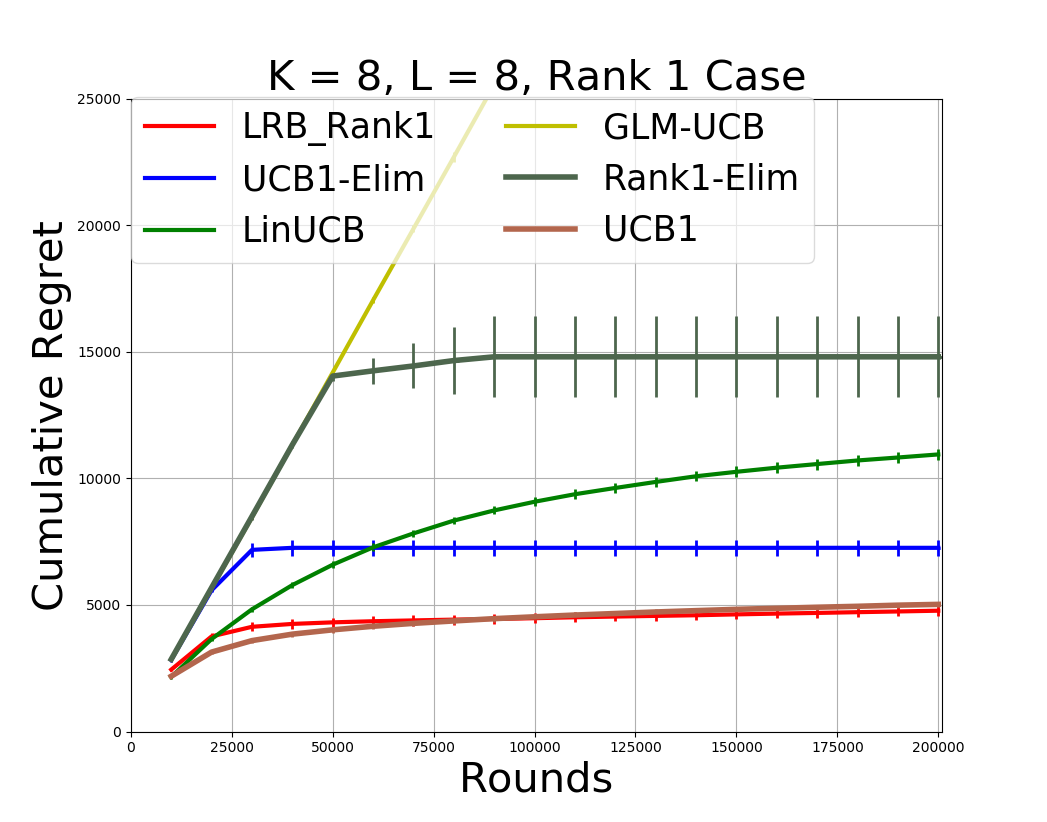
\includegraphics[trim={1cm 0.5cm 1cm 1cm},clip,width=3.7cm]{img/Figure_L1.png}
  		\label{fig:1}
    }
    &
    \hspace*{-1.2em}
    \subfigure[0.22\textwidth][Expt-$1$: $16$ rows, $16$ columns, Rank $1$ Setting]
    %with $r_{i_{{i}\neq {*}}}=0.07$ and $r^{*}=0.1$
    {
    		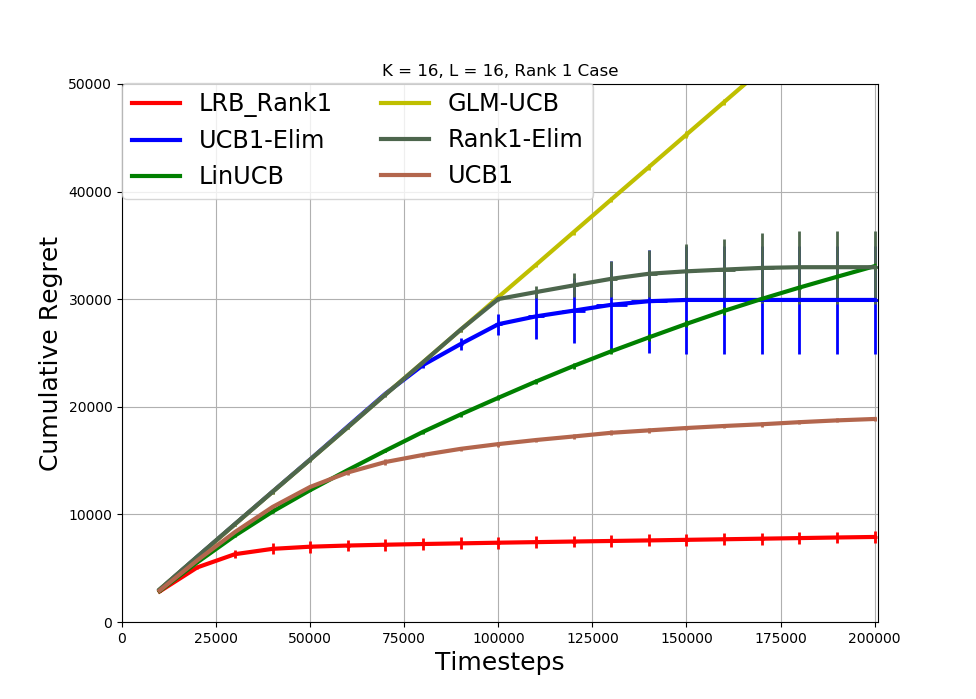
\includegraphics[trim={1cm 0.5cm 1cm 1cm},clip,width=3.7cm]{img/Figure_L2.png}
  		\label{fig:2}
    }
    \\
    \subfigure[0.22\textwidth][Expt-$2$: $64$ rows, $64$ columns, row and column vectors]
    %with $r_{i_{{i}\neq {*}}}=0.07$ and $r^{*}=0.1$
    {
    		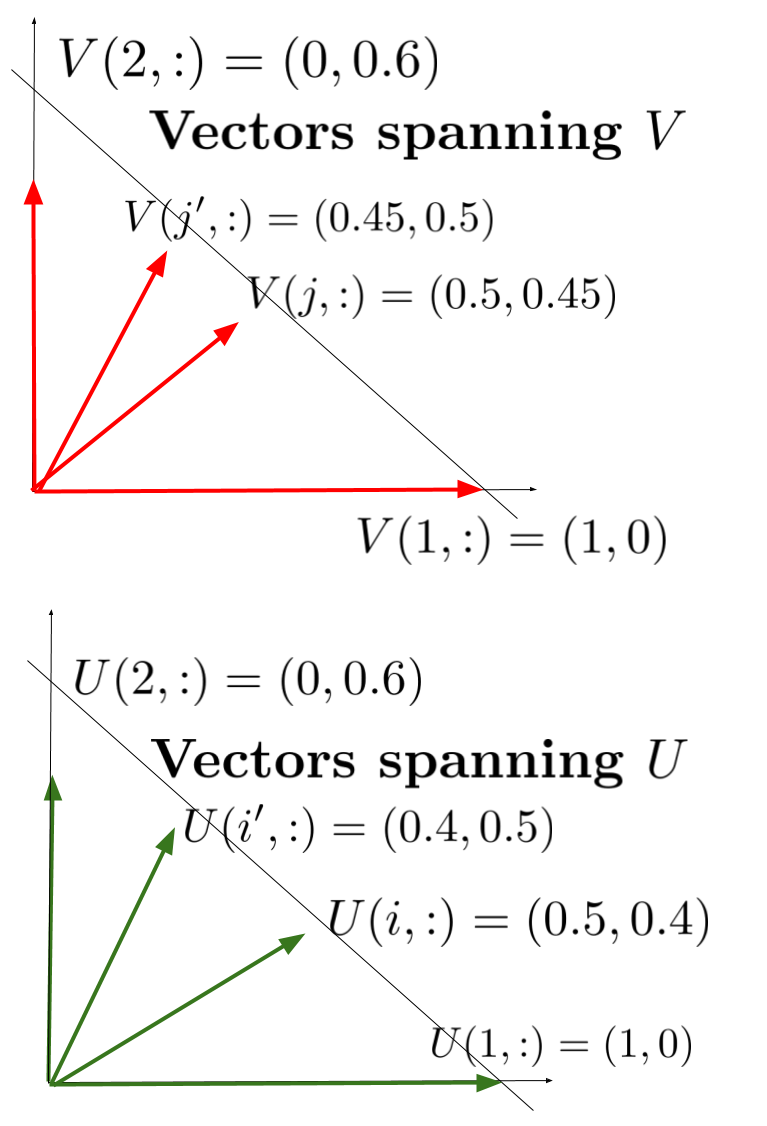
\includegraphics[trim={1cm 1cm 1cm 1cm},clip,width=2.5cm]{img/rank_21_vector.png}
  		\label{fig:3}
    }
    &
     \hspace*{-1.2em}
    \subfigure[0.22\textwidth][Expt-$2$: $64$ rows, $64$ columns, Rank $2$ Setting]
    %with $r_{i_{{i}\neq {*}}}=0.07$ and $r^{*}=0.1$
    {
    		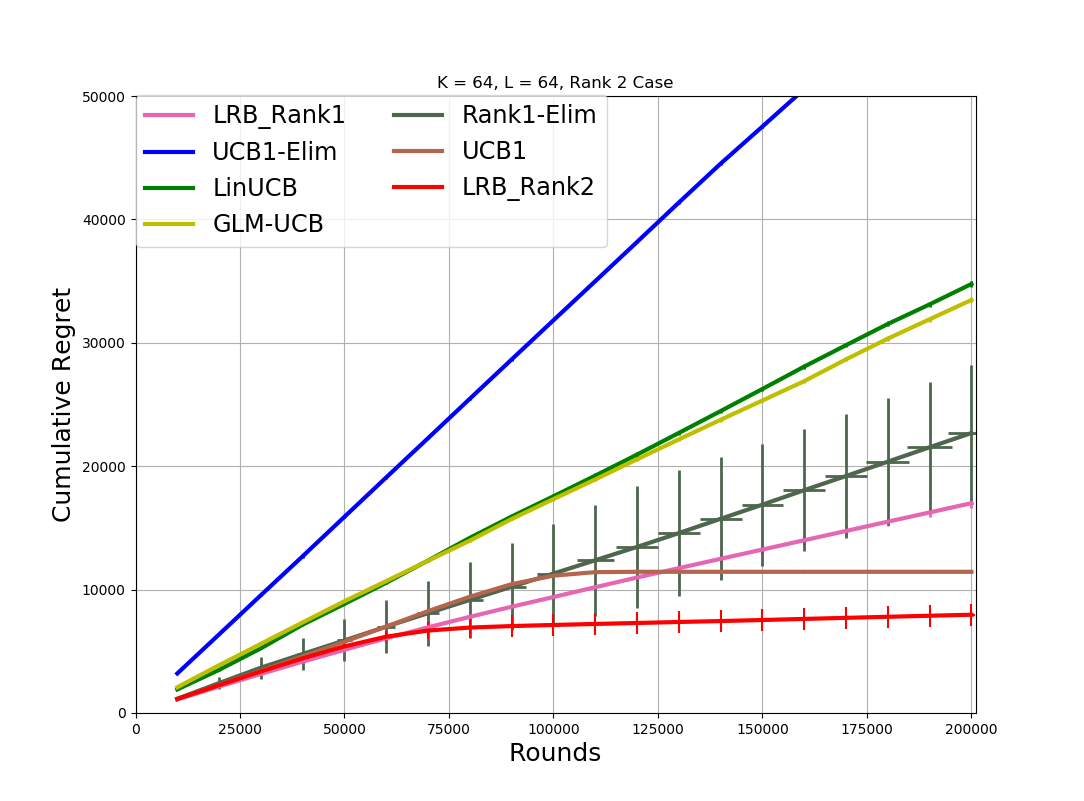
\includegraphics[trim={1cm 0.5cm 1cm 1cm},clip,width=3.9cm]{img/Figure_L3.png}
  		\label{fig:4}
    }
    \end{tabular}
    \caption{A comparison of $\latentranker$ vs state-of-the-art algorithms. }
    \label{fig:karmed1}
    \vspace*{-1.2em}
\end{figure}
%\subsection{Real World Experiment $3$}
\textbf{Real-world Experiment $3$:} We conduct the third experiment to test the performance of $\latentranker$ when our modeling assumptions are violated. We use the Jester dataset \citep{goldberg2001eigentaste} which consist of over 4.1 million continuous ratings of 100 jokes from 73,421 users collected over 5 years. In this dataset there are many users who rated all jokes and we work with these users. 
\begin{wrapfigure}{l}{0.18\textwidth}
    {
            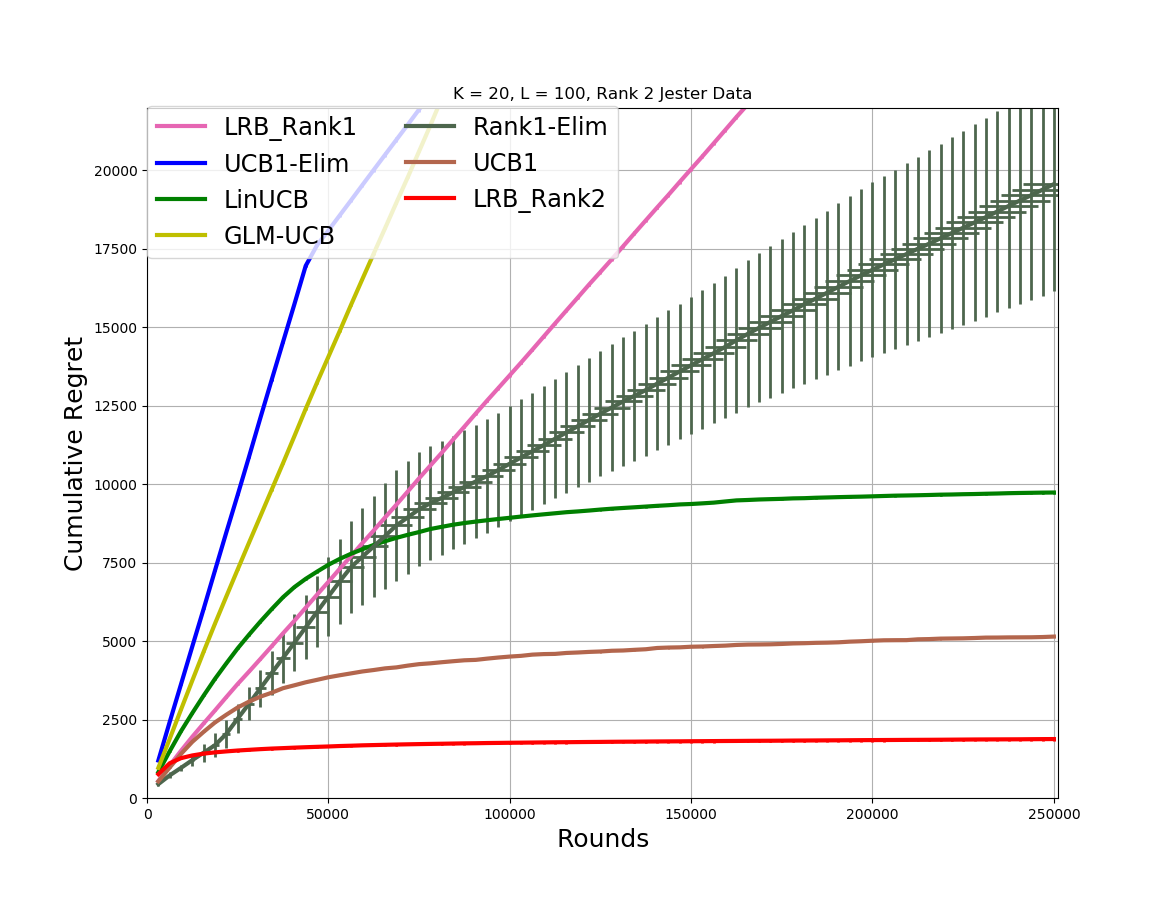
\includegraphics[trim={1cm 1cm 1cm 1cm},clip,width=3.7cm]{img/Figure_L4.png}
   }
 \caption{Expt-$3$: $20$ rows, $100$ columns, Jester Dataset}
 \label{fig:6}
 \vspace{-1.4em}
\end{wrapfigure}
We sample randomly $20$ users (who have rated all jokes) from this dataset and use singular value decomposition (SVD) to obtain a rank $2$ approximation of this user-joke rating matrix $M$. In the resultant matrix $M$, most of the rows belong to the two classes preferring jokes $98$, and $28$, while a very small percentage of users prefer some other jokes. Note that this condition results from the fact that this real-life dataset does not have the hott-topics structure. Furthermore, in this experiment, we assume that the noise is independent Bernoulli over the entries of $M$ and hence this experiment deviates from our modeling assumptions. In Figure \ref{fig:6} we see that $\latentranker$-rank$2$ outperform other algorithms. Finally, $\latentranker$-rank$1$ again fails to perform well in this setting.
%Hence the row-item preference matrix is fully observed and we will not have to complete it using \todoan{You don't have to mention matrix completion here} matrix completion techniques. Hence, this approach is very real world.


%The rank $2$ approximation of $M$ of  is shown in Figure \ref{fig:5}, where we can clearly see the red stripes spanning the matrix indicating the low-rank structure of $M$. 
%\begin{figure}[!th]
%\centering
%\begin{tabular}{cc}
%\setlength{\tabcolsep}{0.1pt}
%\subfigure[0.25\textwidth][Expt-$1$: $500$ Users, $50$ columns, Rank $2$, User and Item vectors]
%    %with $r_{i_{{i}\neq {*}}}=0.07$ and $r^{*}=0.1$
%    {
%    		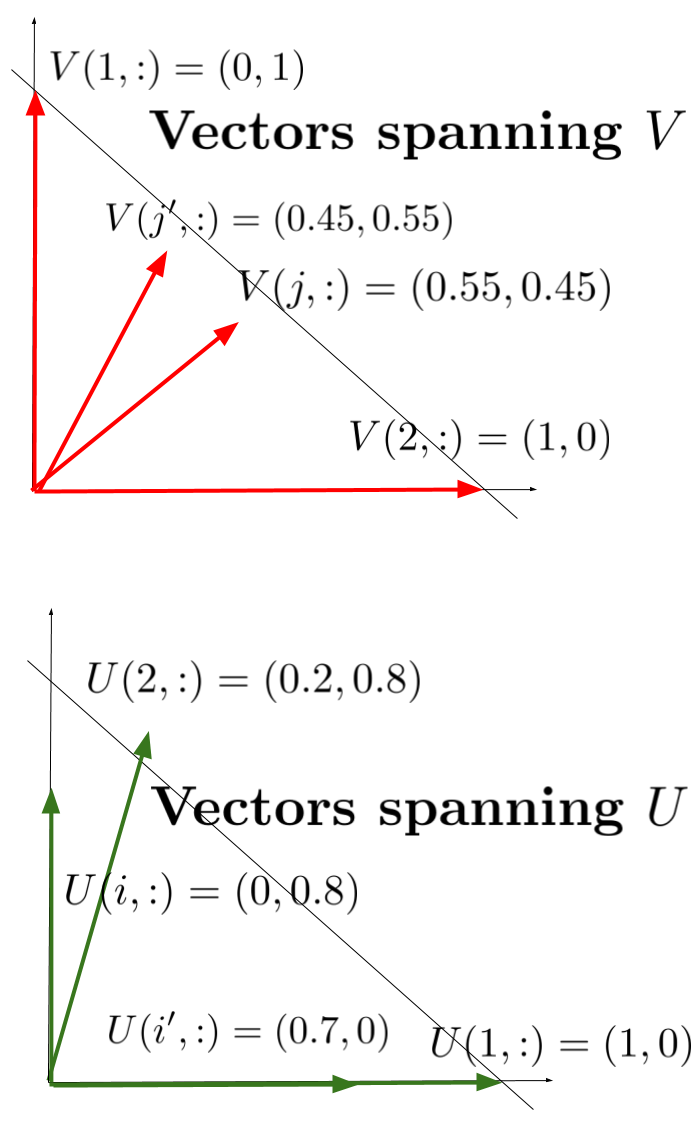
\includegraphics[scale=0.11]{img/rank2_vec.png}
%  		\label{fig:5}
%    }
%    &
%    \subfigure[0.25\textwidth][Expt-$1$: $500$ Users, $50$ columns, Rank $2$, User and Item vectors]
%    %with $r_{i_{{i}\neq {*}}}=0.07$ and $r^{*}=0.1$
%    {
%    		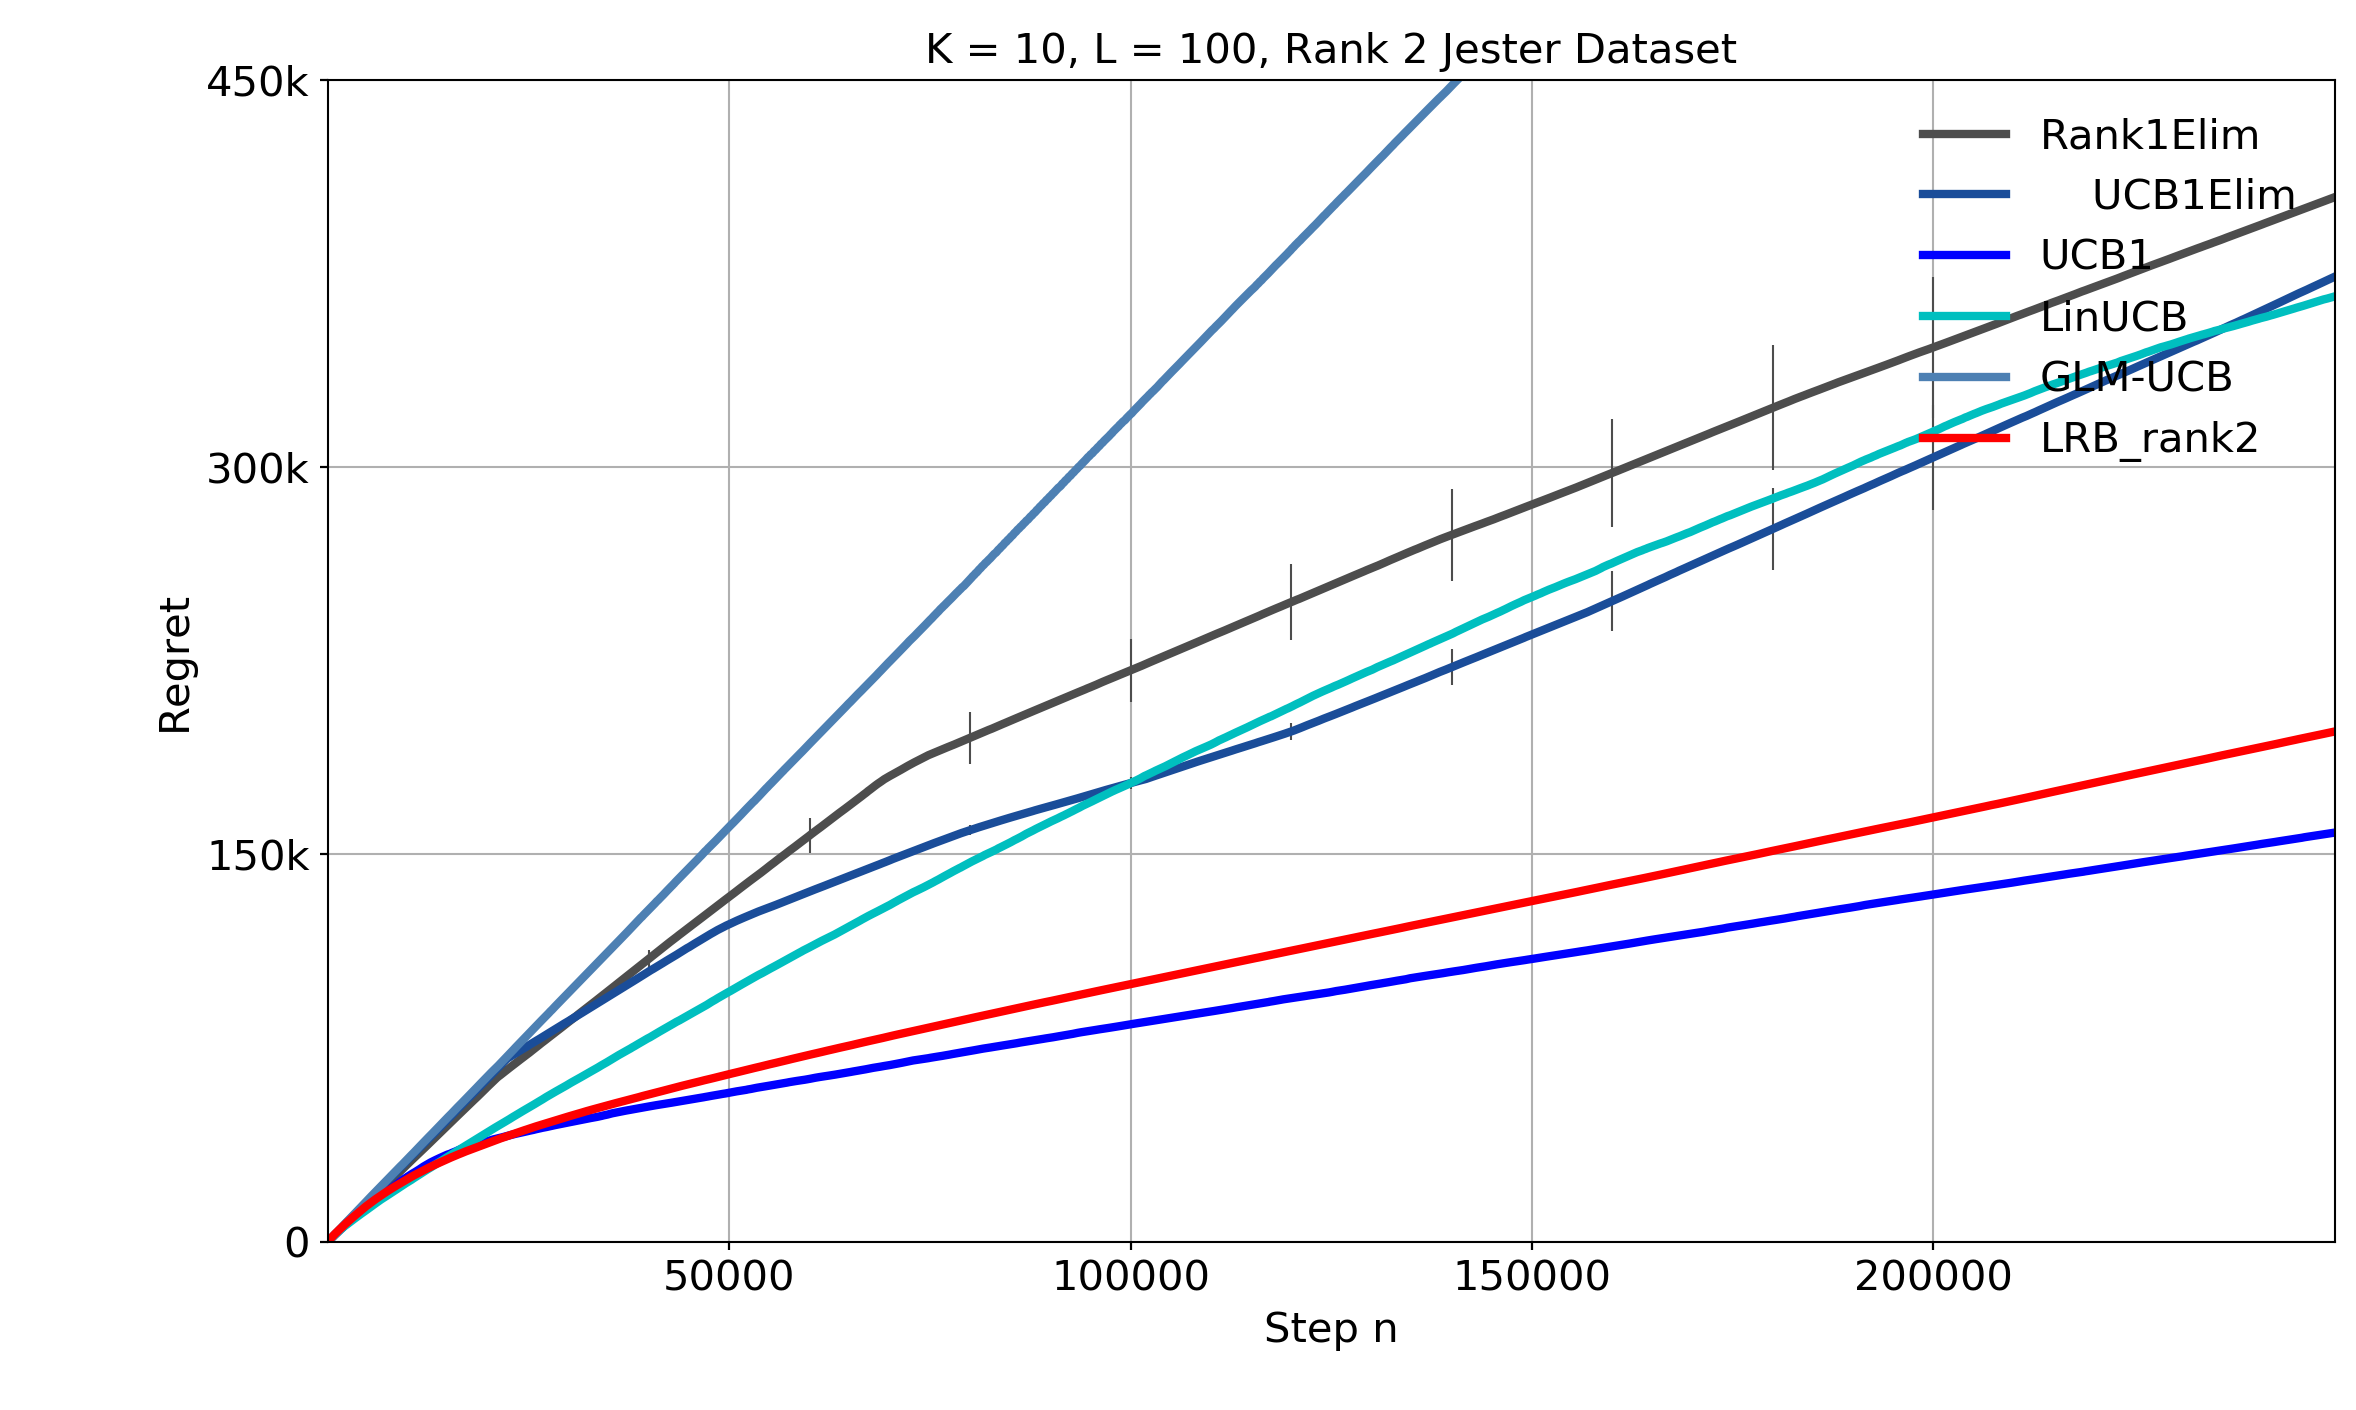
\includegraphics[scale=0.11]{img/Figure_J.png}
%  		\label{fig:1}
%  		\label{fig:6}
%    }
%    \end{tabular}
%    \caption{A comparison of the cumulative regret incurred by the various bandit algorithms. }
%    \label{fig:karmed1}
%    \vspace*{-1em}
%\end{figure}